\subsection{元编程}

\subsection{常见错误处理方法}
由于很多代码都是第三方的,而Rust本身也在不断的发展,有可能出现版本不兼容或者特性
不兼容的情况,此时,则需要进行相关的修改。比如下面的一种错误:
\begin{figure}[H]
  \centering
  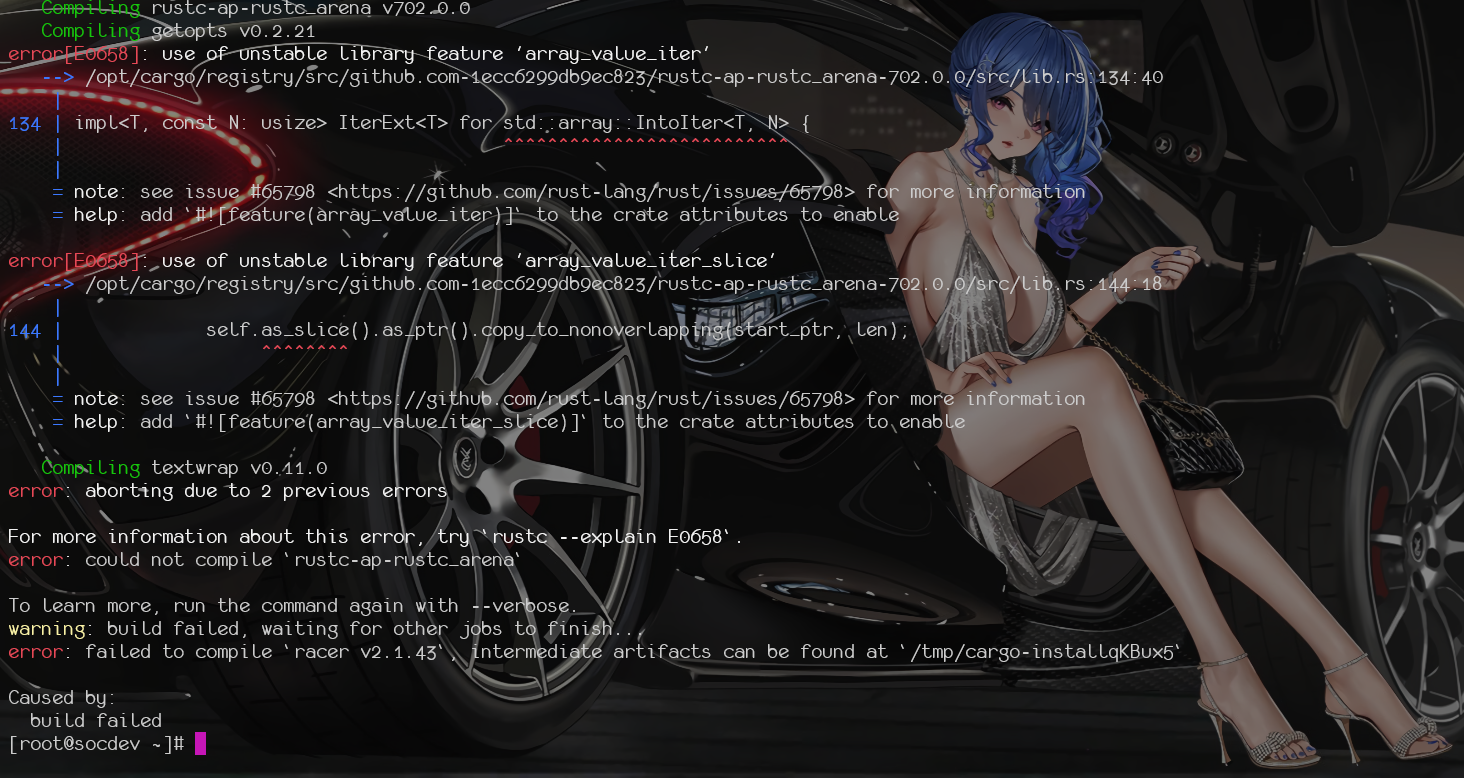
\includegraphics[width=\linewidth]{rust_feature_error.png}
  \caption{缺少特性支持编译失败}
  \label{fig:rust_feature_error}
\end{figure}
遇到这种错误,则需要直接修改对应的类库的源代码。以上述错误为例,编译的help表示
\mintinline[breaklines=true,breakanywhere,breaksymbolleft=,breakanywheresymbolpre=,]{bash}{add `#![feature(array_value_iter_slice)]` to the crate attributes to enable},
则我们应当在对应的crate的lib.rs的头部当中,添加内容如下:
\begin{figure}[H]
  \centering
  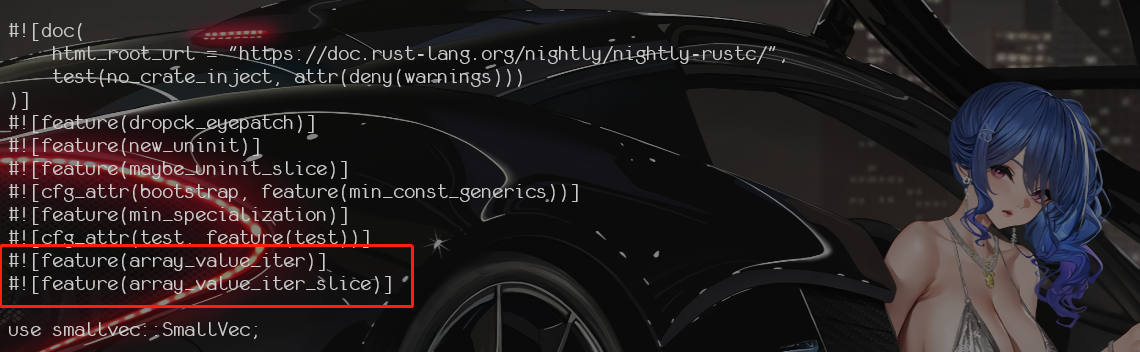
\includegraphics[width=\linewidth]{rust_feature_add.png}
  \caption{增加特性支持}
  \label{fig:rust_feature_add}
\end{figure}
